\subsection{Правила суммы и произведения в комбинаторике. Задачи о подсчете путей. Конечные слова в алфавите. Упорядоченный выбор $k$ элементов из $n$ (с повторениями или без повторений)}

$A$, $B$, $C$ - какие-то конечные множества.
\begin{itemize}
\item \textbf{Правило суммы:}

Пусть $A = B \cup C$ и $B \cap C = \varnothing$, тогда $|A| = |B| + |C|$

\item \textbf{Правило произведения:}

$|A \times B| = |A| \cdot |B|$

\item \textbf{Задача на подсчет путей № 1}

Пусть дана сеточка и вы можете ходить только вправо и вверх по ее узлам. Необходимо посчитать количество путей из левого нижнего угла в правый верхний угол данной сетки.

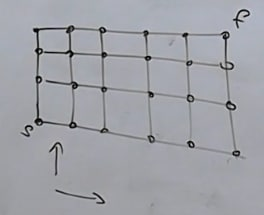
\includegraphics[scale=1.5]{definitions/images/first-patch.jpg}

Можно сделать это, используя, правило суммы. Для каждого из узлов вычисляя количество способов дойти из левого нижнего угла в этот. Для того чтобы насчитать количество путей для очередного узла мы можем просто сложить количество путей ведущих в узел ниже и узел левее. Это верно так как два множества этих путей не пересекаются.

\item \textbf{Задача на подсчет путей № 2}

Найти количество путей из $s$ в $f$ в подобном графе.

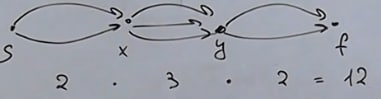
\includegraphics[scale=1.5]{definitions/images/second-patch.jpg}

Множество таких путей можно представить себе как декартово произведение множеств путей между парами вершин.

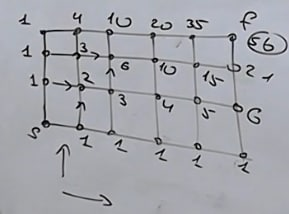
\includegraphics[scale=1.5]{definitions/images/third-patch.png}

Тогда количество путей из $s$ в $f$ это произведение количества путей между парами вершин.

\item \textbf{Упорядоченный выбор $k$ элементов из $n$}

Пусть множество $|A| = n$.

Тогда количество строк длины $k$ с элементами из алфавита $A$ которые могут повторятся, это: $n^k$. То же самое, что количество способов упорядоченно выбрать $k$ элементов из множества размера $n$ с повторениями.

Если же повторения запрещены, то количество таких строк это: $\frac{n!}{(n-k)!}$. То же самое, что количество способов упорядоченно выбрать $k$ элементов из множества размера $n$ без повторений.
\end{itemize}